
\documentclass[border=8pt, multi, tikz]{standalone}
\usepackage{import}
\subimport{layers/}{init}
\usetikzlibrary{positioning}
\usetikzlibrary{3d} %for including external image

\def\ConvColor{rgb:yellow,5;red,2.5;white,5}
\def\ConvReluColor{rgb:yellow,5;red,5;white,5}
\def\PoolColor{rgb:red,1;black,0.3}
\def\UnpoolColor{rgb:blue,2;green,1;black,0.3}
\def\FcColor{rgb:blue,5;red,2.5;white,5}
\def\FcReluColor{rgb:blue,5;red,5;white,4}
\def\SoftmaxColor{rgb:magenta,5;black,7}

\newcommand{\copymidarrow}{\tikz \draw[-Stealth,line width=0.8mm,draw={rgb:blue,4;red,1;green,1;black,3}] (-0.3,0) -- ++(0.3,0);}

\begin{document}
\begin{tikzpicture}
\tikzstyle{connection}=[ultra thick,every node/.style={sloped,allow upside down},draw=\edgecolor,opacity=0.7]
\tikzstyle{copyconnection}=[ultra thick,every node/.style={sloped,allow upside down},draw={rgb:blue,4;red,1;green,1;black,3},opacity=0.7]

\node[canvas is zy plane at x=0][opacity=1] (temp) at (-1,0,0) {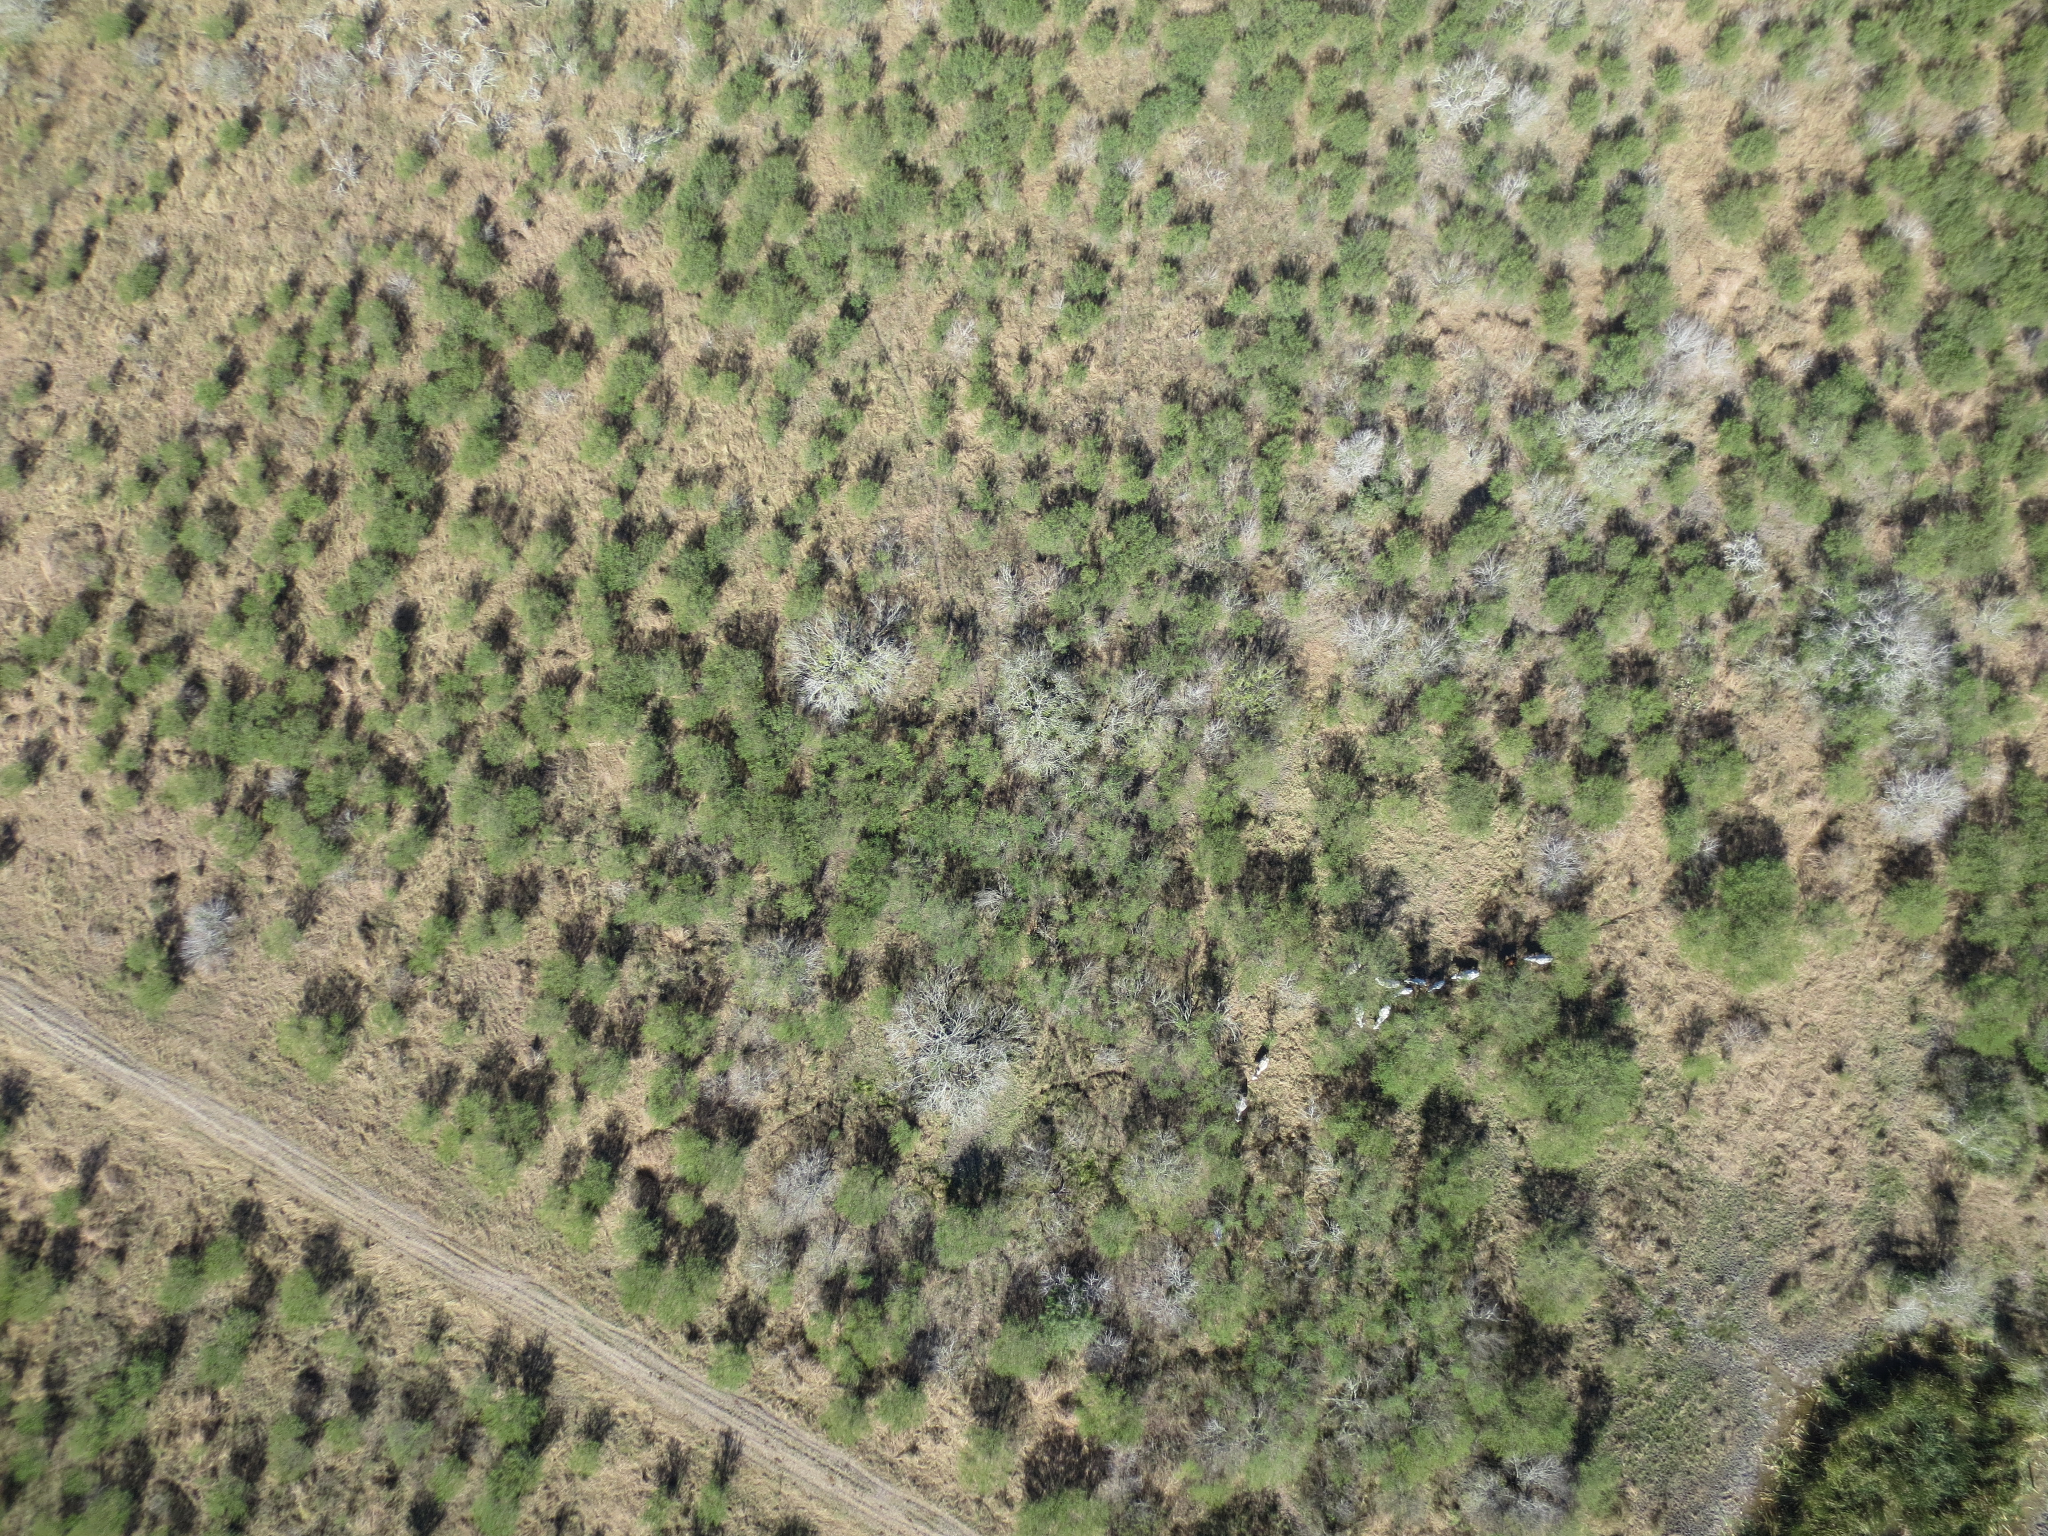
\includegraphics[width=6.826666666666667cm,height=5.120000000000001cm]{IMG_1563_IMG.png}};

\pic[shift={(0,0,0)}] at (0,0,0)
    {Box={
        name=Skip1,
        caption= ,
        xlabel={{16, }},
        zlabel=2048,
        fill=\ConvColor,
        height=25.6,
        width=1,
        depth=34.13333333333333
        }
    };

\pic[shift={ (0,0,0) }] at (Skip1-east)
    {Box={
        name=pool_3,
        caption= ,
        fill=\PoolColor,
        opacity=0.5,
        height=14.287632039711928,
        width=1,
        depth=19.05017605294924
        }
    };

\pic[shift={(1,0,0)}] at (pool_3-east)
    {Box={
        name=conv_4,
        caption= ,
        xlabel={{32, }},
        zlabel=512,
        fill=\ConvColor,
        height=14.287632039711928,
        width=1,
        depth=19.05017605294924
        }
    };

\draw [connection]  (pool_3-east)    -- node {\midarrow} (conv_4-west);

\pic[shift={ (0,0,0) }] at (conv_4-east)
    {Box={
        name=pool_5,
        caption= ,
        fill=\PoolColor,
        opacity=0.5,
        height=7.974079269617299,
        width=1,
        depth=10.632105692823067
        }
    };

\pic[shift={(1,0,0)}] at (pool_5-east)
    {Box={
        name=conv_6,
        caption= ,
        xlabel={{48, }},
        zlabel=128,
        fill=\ConvColor,
        height=7.974079269617299,
        width=1,
        depth=10.632105692823067
        }
    };

\draw [connection]  (pool_5-east)    -- node {\midarrow} (conv_6-west);

\pic[shift={ (0,0,0) }] at (conv_6-east)
    {Box={
        name=pool_7,
        caption= ,
        fill=\PoolColor,
        opacity=0.5,
        height=4.4504183773354224,
        width=1,
        depth=5.933891169780565
        }
    };

\pic[shift={(1,0,0)}] at (pool_7-east)
    {Box={
        name=conv_8,
        caption= ,
        xlabel={{64, }},
        zlabel=32,
        fill=\ConvColor,
        height=4.4504183773354224,
        width=1,
        depth=5.933891169780565
        }
    };

\draw [connection]  (pool_7-east)    -- node {\midarrow} (conv_8-west);

\pic[shift={ (0,0,0) }] at (conv_8-east)
    {Box={
        name=pool_9,
        caption= ,
        fill=\PoolColor,
        opacity=0.5,
        height=3.2102982614314612,
        width=1,
        depth=4.280397681908616
        }
    };

\pic[shift={(1,0,0)}] at (pool_9-east)
    {Box={
        name=END,
        caption= ,
        xlabel={{1, }},
        zlabel=16,
        fill=\ConvColor,
        height=3.2102982614314612,
        width=0.0,
        depth=4.280397681908616
        }
    };

\draw [connection]  (pool_9-east)    -- node {\midarrow} (END-west);

\node[canvas is zy plane at x=0][opacity=0.5] (temp) at (END-east) {\includegraphics[width=0.8560795363817232cm,height=0.6420596522862922cm]{IMG_1563_SPARSE.png}};

\pic[shift={(3,0,0)}] at (END-east)
    {Box={
        name=Sparse,
        caption=Sparse Image,
        xlabel={{3, }},
        zlabel=2048,
        fill=\ConvColor,
        height=25.600000000000005,
        width=1,
        depth=34.13333333333335
        }
    };

\draw [connection]  (END-east)    -- node {\midarrow} (Sparse-west);

\node[canvas is zy plane at x=0][opacity=0.5] (temp) at (Sparse-east) {\includegraphics[width=6.82666666666667cm,height=5.120000000000001cm]{IMG_1563_SPARSE.png}};

\pic[shift={(2,0,0)}] at (Sparse-east)
    {Box={
        name=Skip1,
        caption= ,
        xlabel={{16, }},
        zlabel=2048,
        fill=\ConvColor,
        height=25.600000000000005,
        width=1,
        depth=34.13333333333335
        }
    };

\draw [connection]  (Sparse-east)    -- node {\midarrow} (Skip1-west);

\pic[shift={ (0,0,0) }] at (Skip1-east)
    {Box={
        name=pool_19,
        caption= ,
        fill=\PoolColor,
        opacity=0.5,
        height=18.466496523378737,
        width=1,
        depth=24.62199536450499
        }
    };

\pic[shift={(1,0,0)}] at (pool_19-east)
    {Box={
        name=Skip2,
        caption= ,
        xlabel={{32, }},
        zlabel=1024,
        fill=\ConvColor,
        height=18.466496523378737,
        width=1,
        depth=24.62199536450499
        }
    };

\draw [connection]  (pool_19-east)    -- node {\midarrow} (Skip2-west);

\pic[shift={ (0,0,0) }] at (Skip2-east)
    {Box={
        name=pool_21,
        caption= ,
        fill=\PoolColor,
        opacity=0.5,
        height=13.320761478435895,
        width=1,
        depth=17.761015304581196
        }
    };

\pic[shift={(1,0,0)}] at (pool_21-east)
    {Box={
        name=Skip3,
        caption= ,
        xlabel={{48, }},
        zlabel=512,
        fill=\ConvColor,
        height=13.320761478435895,
        width=1,
        depth=17.761015304581196
        }
    };

\draw [connection]  (pool_21-east)    -- node {\midarrow} (Skip3-west);

\pic[shift={ (0,0,0) }] at (Skip3-east)
    {Box={
        name=pool_23,
        caption= ,
        fill=\PoolColor,
        opacity=0.5,
        height=9.608898262902102,
        width=1,
        depth=12.811864350536137
        }
    };

\pic[shift={(1,0,0)}] at (pool_23-east)
    {Box={
        name=Skip4,
        caption= ,
        xlabel={{64, }},
        zlabel=256,
        fill=\ConvColor,
        height=9.608898262902102,
        width=1,
        depth=12.811864350536137
        }
    };

\draw [connection]  (pool_23-east)    -- node {\midarrow} (Skip4-west);

\pic[shift={ (0,0,0) }] at (Skip4-east)
    {Box={
        name=pool_25,
        caption= ,
        fill=\PoolColor,
        opacity=0.5,
        height=6.931354936147718,
        width=1,
        depth=9.241806581530295
        }
    };

\pic[shift={(1,0,0)}] at (pool_25-east)
    {Box={
        name=conv_26,
        caption= ,
        xlabel={{80, }},
        zlabel=128,
        fill=\ConvColor,
        height=6.931354936147718,
        width=1,
        depth=9.241806581530295
        }
    };

\draw [connection]  (pool_25-east)    -- node {\midarrow} (conv_26-west);

\pic[shift={ (1,0,0) }] at (conv_26-east)
    {Box={
        name=Dest4,
        caption= ,
        xlabel={{64, }},
        zlabel=256,
        fill=\UnpoolColor,
        opacity=0.5,
        height=9.608898262902102,
        width=1,
        depth=12.81186435053614
        }
    };

\draw [connection]  (conv_26-east)    -- node {\midarrow} (Dest4-west);

\path (Skip4-southeast) -- (Skip4-northeast) coordinate[pos=1.25] (Skip4-top) ;
\path (Dest4-south)  -- (Dest4-north)  coordinate[pos=1.25] (Dest4-top) ;
\draw [copyconnection]  (Skip4-northeast)
-- node {\copymidarrow}(Skip4-top)
-- node {\copymidarrow}(Dest4-top)
-- node {\copymidarrow} (Dest4-north);

\pic[shift={ (1,0,0) }] at (Dest4-east)
    {Box={
        name=Dest3,
        caption= ,
        xlabel={{32, }},
        zlabel=512,
        fill=\UnpoolColor,
        opacity=0.5,
        height=13.320761478435895,
        width=1,
        depth=17.7610153045812
        }
    };

\draw [connection]  (Dest4-east)    -- node {\midarrow} (Dest3-west);

\path (Skip3-southeast) -- (Skip3-northeast) coordinate[pos=1.25] (Skip3-top) ;
\path (Dest3-south)  -- (Dest3-north)  coordinate[pos=1.25] (Dest3-top) ;
\draw [copyconnection]  (Skip3-northeast)
-- node {\copymidarrow}(Skip3-top)
-- node {\copymidarrow}(Dest3-top)
-- node {\copymidarrow} (Dest3-north);

\pic[shift={ (1,0,0) }] at (Dest3-east)
    {Box={
        name=Dest2,
        caption= ,
        xlabel={{16, }},
        zlabel=1024,
        fill=\UnpoolColor,
        opacity=0.5,
        height=18.46649652337874,
        width=1,
        depth=24.621995364504997
        }
    };

\draw [connection]  (Dest3-east)    -- node {\midarrow} (Dest2-west);

\path (Skip2-southeast) -- (Skip2-northeast) coordinate[pos=1.25] (Skip2-top) ;
\path (Dest2-south)  -- (Dest2-north)  coordinate[pos=1.25] (Dest2-top) ;
\draw [copyconnection]  (Skip2-northeast)
-- node {\copymidarrow}(Skip2-top)
-- node {\copymidarrow}(Dest2-top)
-- node {\copymidarrow} (Dest2-north);

\pic[shift={ (1,0,0) }] at (Dest2-east)
    {Box={
        name=Dest1,
        caption= ,
        xlabel={{8, }},
        zlabel=2048,
        fill=\UnpoolColor,
        opacity=0.5,
        height=25.600000000000012,
        width=1,
        depth=34.13333333333337
        }
    };

\draw [connection]  (Dest2-east)    -- node {\midarrow} (Dest1-west);

\path (Skip1-southeast) -- (Skip1-northeast) coordinate[pos=1.25] (Skip1-top) ;
\path (Dest1-south)  -- (Dest1-north)  coordinate[pos=1.25] (Dest1-top) ;
\draw [copyconnection]  (Skip1-northeast)
-- node {\copymidarrow}(Skip1-top)
-- node {\copymidarrow}(Dest1-top)
-- node {\copymidarrow} (Dest1-north);

\pic[shift={(1,0,0)}] at (Dest1-east)
    {Box={
        name=END2,
        caption=Probability Heat Map,
        xlabel={{1, }},
        zlabel=2048,
        fill=\ConvColor,
        height=25.600000000000012,
        width=0.0,
        depth=34.13333333333337
        }
    };

\draw [connection]  (Dest1-east)    -- node {\midarrow} (END2-west);

\node[canvas is zy plane at x=0][opacity=0.5] (temp) at (END2-east) {\includegraphics[width=6.826666666666674cm,height=5.120000000000003cm]{IMG_1563_ANN.png}};

\end{tikzpicture}
\end{document}
